\documentclass[12pt letter]{report}
%%%%%%%%%%%%%%%%%%%%%%%%%%%%%%%%%
% PACKAGE IMPORTS
%%%%%%%%%%%%%%%%%%%%%%%%%%%%%%%%%


\usepackage[tmargin=2cm,rmargin=1in,lmargin=1in,margin=0.85in,bmargin=2cm,footskip=.2in]{geometry}
\usepackage{amsmath,amsfonts,amsthm,amssymb,mathtools}
\usepackage[varbb]{newpxmath}
\usepackage{xfrac}
\usepackage[makeroom]{cancel}
\usepackage{mathtools}
\usepackage{bookmark}
\usepackage{enumitem}
\usepackage{hyperref,theoremref}
\hypersetup{
  pdftitle={Assignment},
  colorlinks=true, linkcolor=doc!90,
  bookmarksnumbered=true,
  bookmarksopen=true
}
\usepackage[most,many,breakable]{tcolorbox}
\usepackage{xcolor}
\usepackage{varwidth}
\usepackage{varwidth}
\usepackage{etoolbox}
%\usepackage{authblk}
\usepackage{nameref}
\usepackage{multicol,array}
\usepackage{tikz-cd}
\usepackage[ruled,vlined,linesnumbered]{algorithm2e}
\usepackage{comment} % enables the use of multi-line comments (\ifx \fi) 
\usepackage{import}
\usepackage{xifthen}
\usepackage{pdfpages}
\usepackage{transparent}
\usepackage{xcolor,colortbl,array,amssymb}
\usepackage{venndiagram}
\usepackage{listings}
\usepackage{fontspec}

\setmainfont{LibertinusSerif}[
  Extension = .otf,
  Path = /usr/share/fonts/libertinus/,
  UprightFont = *-Regular,
  ItalicFont = *-Italic,
  BoldFont = *-Bold,
  BoldItalicFont = *-BoldItalic,
]

\setmonofont{CaskaydiaCoveNerdFontMono}[
  Extension = .ttf,
  Path = /usr/share/fonts/TTF/,
  UprightFont = *-Regular,
  ItalicFont = *-Italic,
  BoldFont = *-Bold,
  BoldItalicFont = *-BoldItalic,
]

\definecolor{listing-background}{HTML}{F7F7F7}
\definecolor{listing-rule}{HTML}{B3B2B3}
\definecolor{listing-numbers}{HTML}{B3B2B3}
\definecolor{listing-text-color}{HTML}{000000}
\definecolor{listing-keyword}{HTML}{435489}
\definecolor{listing-keyword-2}{HTML}{1284CA} % additional keywords
\definecolor{listing-keyword-3}{HTML}{9137CB} % additional keywords
\definecolor{listing-identifier}{HTML}{435489}
\definecolor{listing-string}{HTML}{00999A}
\definecolor{listing-comment}{HTML}{8E8E8E}

\lstdefinestyle{eisvogel_listing_style}{
language         = java,
xleftmargin      = 0.6em,
framexleftmargin = 0.4em,
backgroundcolor  = \color{listing-background},
basicstyle       = \color{listing-text-color}\linespread{1.0}%
\lst@ifdisplaystyle%
\fi\ttfamily{},
breaklines       = true,
frame            = single,
framesep         = 0.19em,
rulecolor        = \color{listing-rule},
frameround       = ffff,
tabsize          = 4,
numberstyle      = \color{listing-numbers},
aboveskip        = 1.0em,
belowskip        = 0.1em,
abovecaptionskip = 0em,
belowcaptionskip = 1.0em,
keywordstyle     = {\color{listing-keyword}\bfseries},
keywordstyle     = {[2]\color{listing-keyword-2}\bfseries},
keywordstyle     = {[3]\color{listing-keyword-3}\bfseries\itshape},
sensitive        = true,
identifierstyle  = \color{listing-identifier},
commentstyle     = \color{listing-comment},
stringstyle      = \color{listing-string},
showstringspaces = false,
escapeinside     = {/*@}{@*/}, % Allow LaTeX inside these special comments
literate         =
  {á}{{\'a}}1 {é}{{\'e}}1 {í}{{\'i}}1 {ó}{{\'o}}1 {ú}{{\'u}}1
{Á}{{\'A}}1 {É}{{\'E}}1 {Í}{{\'I}}1 {Ó}{{\'O}}1 {Ú}{{\'U}}1
{à}{{\`a}}1 {è}{{\`e}}1 {ì}{{\`i}}1 {ò}{{\`o}}1 {ù}{{\`u}}1
{À}{{\`A}}1 {È}{{\`E}}1 {Ì}{{\`I}}1 {Ò}{{\`O}}1 {Ù}{{\`U}}1
{ä}{{\"a}}1 {ë}{{\"e}}1 {ï}{{\"i}}1 {ö}{{\"o}}1 {ü}{{\"u}}1
{Ä}{{\"A}}1 {Ë}{{\"E}}1 {Ï}{{\"I}}1 {Ö}{{\"O}}1 {Ü}{{\"U}}1
{â}{{\^a}}1 {ê}{{\^e}}1 {î}{{\^i}}1 {ô}{{\^o}}1 {û}{{\^u}}1
{Â}{{\^A}}1 {Ê}{{\^E}}1 {Î}{{\^I}}1 {Ô}{{\^O}}1 {Û}{{\^U}}1
{œ}{{\oe}}1 {Œ}{{\OE}}1 {æ}{{\ae}}1 {Æ}{{\AE}}1 {ß}{{\ss}}1
{ç}{{\c c}}1 {Ç}{{\c C}}1 {ø}{{\o}}1 {å}{{\r a}}1 {Å}{{\r A}}1
{€}{{\EUR}}1 {£}{{\pounds}}1 {«}{{\guillemotleft}}1
{»}{{\guillemotright}}1 {ñ}{{\~n}}1 {Ñ}{{\~N}}1 {¿}{{?`}}1
{…}{{\ldots}}1 {≥}{{>=}}1 {≤}{{<=}}1 {„}{{\glqq}}1 {“}{{\grqq}}1
{”}{{''}}1
}
\lstset{style=eisvogel_listing_style,
  numbers=left}

%
% Java (Java SE 12, 2019-06-22)
%
\lstdefinelanguage{Java}{
  morekeywords={
      % normal keywords (without data types)
      abstract,assert,break,case,catch,class,continue,default,
      do,else,enum,exports,extends,final,finally,for,if,implements,
      import,instanceof,interface,module,native,new,package,private,
      protected,public,requires,return,static,strictfp,super,switch,
      synchronized,this,throw,throws,transient,try,volatile,while,
      % var is an identifier
      var
    },
  morekeywords={[2] % data types
      % primitive data types
      boolean,byte,char,double,float,int,long,short,
      % String
      String,
      % primitive wrapper types
      Boolean,Byte,Character,Double,Float,Integer,Long,Short
      % number types
      Number,AtomicInteger,AtomicLong,BigDecimal,BigInteger,DoubleAccumulator,DoubleAdder,LongAccumulator,LongAdder,Short,
      % other
      Object,Void,void
    },
  morekeywords={[3] % literals
      % reserved words for literal values
      null,true,false,
    },
  sensitive,
  morecomment  = [l]//,
  morecomment  = [s]{/*}{*/},
  morecomment  = [s]{/**}{*/},
  morestring   = [b]",
  morestring   = [b]',
}

\lstdefinelanguage{XML}{
  morestring      = [b]",
  moredelim       = [s][\bfseries\color{listing-keyword}]{<}{\ },
  moredelim       = [s][\bfseries\color{listing-keyword}]{</}{>},
  moredelim       = [l][\bfseries\color{listing-keyword}]{/>},
  moredelim       = [l][\bfseries\color{listing-keyword}]{>},
  morecomment     = [s]{<?}{?>},
  morecomment     = [s]{<!--}{-->},
  commentstyle    = \color{listing-comment},
  stringstyle     = \color{listing-string},
  identifierstyle = \color{listing-identifier}
}


\newcommand\mycommfont[1]{\footnotesize\ttfamily\textcolor{blue}{#1}}
\SetCommentSty{mycommfont}
\newcommand{\incfig}[1]{%
  \def\svgwidth{\columnwidth}
  \import{./figures/}{#1.pdf_tex}
}

\usepackage{tikzsymbols}
\renewcommand\qedsymbol{$\Laughey$}


%\usepackage{import}
%\usepackage{xifthen}
%\usepackage{pdfpages}
%\usepackage{transparent}


%%%%%%%%%%%%%%%%%%%%%%%%%%%%%%
% SELF MADE COLORS
%%%%%%%%%%%%%%%%%%%%%%%%%%%%%%



\definecolor{myg}{RGB}{56, 140, 70}
\definecolor{myb}{RGB}{45, 111, 177}
\definecolor{myr}{RGB}{199, 68, 64}
\definecolor{mytheorembg}{HTML}{F2F2F9}
\definecolor{mytheoremfr}{HTML}{00007B}
\definecolor{mylenmabg}{HTML}{FFFAF8}
\definecolor{mylenmafr}{HTML}{983b0f}
\definecolor{mypropbg}{HTML}{f2fbfc}
\definecolor{mypropfr}{HTML}{191971}
\definecolor{myexamplebg}{HTML}{F2FBF8}
\definecolor{myexamplefr}{HTML}{88D6D1}
\definecolor{myexampleti}{HTML}{2A7F7F}
\definecolor{mydefinitbg}{HTML}{E5E5FF}
\definecolor{mydefinitfr}{HTML}{3F3FA3}
\definecolor{notesgreen}{RGB}{0,162,0}
\definecolor{myp}{RGB}{197, 92, 212}
\definecolor{mygr}{HTML}{2C3338}
\definecolor{myred}{RGB}{127,0,0}
\definecolor{myyellow}{RGB}{169,121,69}
\definecolor{myexercisebg}{HTML}{F2FBF8}
\definecolor{myexercisefg}{HTML}{88D6D1}


%%%%%%%%%%%%%%%%%%%%%%%%%%%%
% TCOLORBOX SETUPS
%%%%%%%%%%%%%%%%%%%%%%%%%%%%

\setlength{\parindent}{1cm}
%================================
% THEOREM BOX
%================================

\tcbuselibrary{theorems,skins,hooks}
\newtcbtheorem[number within=section]{Theorem}{Theorem}
{%
  enhanced,
  breakable,
  colback = mytheorembg,
  frame hidden,
  boxrule = 0sp,
  borderline west = {2pt}{0pt}{mytheoremfr},
  sharp corners,
  detach title,
  before upper = \tcbtitle\par\smallskip,
  coltitle = mytheoremfr,
  fonttitle = \bfseries\sffamily,
  description font = \mdseries,
  separator sign none,
  segmentation style={solid, mytheoremfr},
}
{th}

\tcbuselibrary{theorems,skins,hooks}
\newtcbtheorem[number within=chapter]{theorem}{Theorem}
{%
  enhanced,
  breakable,
  colback = mytheorembg,
  frame hidden,
  boxrule = 0sp,
  borderline west = {2pt}{0pt}{mytheoremfr},
  sharp corners,
  detach title,
  before upper = \tcbtitle\par\smallskip,
  coltitle = mytheoremfr,
  fonttitle = \bfseries\sffamily,
  description font = \mdseries,
  separator sign none,
  segmentation style={solid, mytheoremfr},
}
{th}


\tcbuselibrary{theorems,skins,hooks}
\newtcolorbox{Theoremcon}
{%
  enhanced
  ,breakable
  ,colback = mytheorembg
  ,frame hidden
  ,boxrule = 0sp
  ,borderline west = {2pt}{0pt}{mytheoremfr}
  ,sharp corners
  ,description font = \mdseries
  ,separator sign none
}

%================================
% Corollery
%================================
\tcbuselibrary{theorems,skins,hooks}
\newtcbtheorem[number within=section]{Corollary}{Corollary}
{%
  enhanced
  ,breakable
  ,colback = myp!10
  ,frame hidden
  ,boxrule = 0sp
  ,borderline west = {2pt}{0pt}{myp!85!black}
  ,sharp corners
  ,detach title
  ,before upper = \tcbtitle\par\smallskip
  ,coltitle = myp!85!black
  ,fonttitle = \bfseries\sffamily
  ,description font = \mdseries
  ,separator sign none
  ,segmentation style={solid, myp!85!black}
}
{th}
\tcbuselibrary{theorems,skins,hooks}
\newtcbtheorem[number within=chapter]{corollary}{Corollary}
{%
  enhanced
  ,breakable
  ,colback = myp!10
  ,frame hidden
  ,boxrule = 0sp
  ,borderline west = {2pt}{0pt}{myp!85!black}
  ,sharp corners
  ,detach title
  ,before upper = \tcbtitle\par\smallskip
  ,coltitle = myp!85!black
  ,fonttitle = \bfseries\sffamily
  ,description font = \mdseries
  ,separator sign none
  ,segmentation style={solid, myp!85!black}
}
{th}


%================================
% LENMA
%================================

\tcbuselibrary{theorems,skins,hooks}
\newtcbtheorem[number within=section]{Lenma}{Lenma}
{%
  enhanced,
  breakable,
  colback = mylenmabg,
  frame hidden,
  boxrule = 0sp,
  borderline west = {2pt}{0pt}{mylenmafr},
  sharp corners,
  detach title,
  before upper = \tcbtitle\par\smallskip,
  coltitle = mylenmafr,
  fonttitle = \bfseries\sffamily,
  description font = \mdseries,
  separator sign none,
  segmentation style={solid, mylenmafr},
}
{th}

\tcbuselibrary{theorems,skins,hooks}
\newtcbtheorem[number within=chapter]{lenma}{Lenma}
{%
  enhanced,
  breakable,
  colback = mylenmabg,
  frame hidden,
  boxrule = 0sp,
  borderline west = {2pt}{0pt}{mylenmafr},
  sharp corners,
  detach title,
  before upper = \tcbtitle\par\smallskip,
  coltitle = mylenmafr,
  fonttitle = \bfseries\sffamily,
  description font = \mdseries,
  separator sign none,
  segmentation style={solid, mylenmafr},
}
{th}


%================================
% PROPOSITION
%================================

\tcbuselibrary{theorems,skins,hooks}
\newtcbtheorem[number within=section]{Prop}{Proposition}
{%
  enhanced,
  breakable,
  colback = mypropbg,
  frame hidden,
  boxrule = 0sp,
  borderline west = {2pt}{0pt}{mypropfr},
  sharp corners,
  detach title,
  before upper = \tcbtitle\par\smallskip,
  coltitle = mypropfr,
  fonttitle = \bfseries\sffamily,
  description font = \mdseries,
  separator sign none,
  segmentation style={solid, mypropfr},
}
{th}

\tcbuselibrary{theorems,skins,hooks}
\newtcbtheorem[number within=chapter]{prop}{Proposition}
{%
  enhanced,
  breakable,
  colback = mypropbg,
  frame hidden,
  boxrule = 0sp,
  borderline west = {2pt}{0pt}{mypropfr},
  sharp corners,
  detach title,
  before upper = \tcbtitle\par\smallskip,
  coltitle = mypropfr,
  fonttitle = \bfseries\sffamily,
  description font = \mdseries,
  separator sign none,
  segmentation style={solid, mypropfr},
}
{th}


%================================
% CLAIM
%================================

\tcbuselibrary{theorems,skins,hooks}
\newtcbtheorem[number within=section]{claim}{Claim}
{%
  enhanced
  ,breakable
  ,colback = myg!10
  ,frame hidden
  ,boxrule = 0sp
  ,borderline west = {2pt}{0pt}{myg}
  ,sharp corners
  ,detach title
  ,before upper = \tcbtitle\par\smallskip
  ,coltitle = myg!85!black
  ,fonttitle = \bfseries\sffamily
  ,description font = \mdseries
  ,separator sign none
  ,segmentation style={solid, myg!85!black}
}
{th}



%================================
% Exercise
%================================

\tcbuselibrary{theorems,skins,hooks}
\newtcbtheorem[number within=section]{Exercise}{Exercise}
{%
  enhanced,
  breakable,
  colback = myexercisebg,
  frame hidden,
  boxrule = 0sp,
  borderline west = {2pt}{0pt}{myexercisefg},
  sharp corners,
  detach title,
  before upper = \tcbtitle\par\smallskip,
  coltitle = myexercisefg,
  fonttitle = \bfseries\sffamily,
  description font = \mdseries,
  separator sign none,
  segmentation style={solid, myexercisefg},
}
{th}

\tcbuselibrary{theorems,skins,hooks}
\newtcbtheorem[number within=chapter]{exercise}{Exercise}
{%
  enhanced,
  breakable,
  colback = myexercisebg,
  frame hidden,
  boxrule = 0sp,
  borderline west = {2pt}{0pt}{myexercisefg},
  sharp corners,
  detach title,
  before upper = \tcbtitle\par\smallskip,
  coltitle = myexercisefg,
  fonttitle = \bfseries\sffamily,
  description font = \mdseries,
  separator sign none,
  segmentation style={solid, myexercisefg},
}
{th}

%================================
% EXAMPLE BOX
%================================

\newtcbtheorem[number within=section]{Example}{Example}
{%
  colback = myexamplebg
  ,breakable
  ,colframe = myexamplefr
  ,coltitle = myexampleti
  ,boxrule = 1pt
  ,sharp corners
  ,detach title
  ,before upper=\tcbtitle\par\smallskip
  ,fonttitle = \bfseries
  ,description font = \mdseries
  ,separator sign none
  ,description delimiters parenthesis
}
{ex}

\newtcbtheorem[number within=chapter]{example}{Example}
{%
  colback = myexamplebg
  ,breakable
  ,colframe = myexamplefr
  ,coltitle = myexampleti
  ,boxrule = 1pt
  ,sharp corners
  ,detach title
  ,before upper=\tcbtitle\par\smallskip
  ,fonttitle = \bfseries
  ,description font = \mdseries
  ,separator sign none
  ,description delimiters parenthesis
}
{ex}

%================================
% DEFINITION BOX
%================================

\newtcbtheorem[number within=section]{Definition}{Definition}{enhanced,
  before skip=2mm,after skip=2mm, colback=red!5,colframe=red!80!black,boxrule=0.5mm,
  attach boxed title to top left={xshift=1cm,yshift*=1mm-\tcboxedtitleheight}, varwidth boxed title*=-3cm,
  boxed title style={frame code={
          \path[fill=tcbcolback]
          ([yshift=-1mm,xshift=-1mm]frame.north west)
          arc[start angle=0,end angle=180,radius=1mm]
          ([yshift=-1mm,xshift=1mm]frame.north east)
          arc[start angle=180,end angle=0,radius=1mm];
          \path[left color=tcbcolback!60!black,right color=tcbcolback!60!black,
            middle color=tcbcolback!80!black]
          ([xshift=-2mm]frame.north west) -- ([xshift=2mm]frame.north east)
          [rounded corners=1mm]-- ([xshift=1mm,yshift=-1mm]frame.north east)
          -- (frame.south east) -- (frame.south west)
          -- ([xshift=-1mm,yshift=-1mm]frame.north west)
          [sharp corners]-- cycle;
        },interior engine=empty,
    },
  fonttitle=\bfseries,
  title={#2},#1}{def}
\newtcbtheorem[number within=chapter]{definition}{Definition}{enhanced,
  before skip=2mm,after skip=2mm, colback=red!5,colframe=red!80!black,boxrule=0.5mm,
  attach boxed title to top left={xshift=1cm,yshift*=1mm-\tcboxedtitleheight}, varwidth boxed title*=-3cm,
  boxed title style={frame code={
          \path[fill=tcbcolback]
          ([yshift=-1mm,xshift=-1mm]frame.north west)
          arc[start angle=0,end angle=180,radius=1mm]
          ([yshift=-1mm,xshift=1mm]frame.north east)
          arc[start angle=180,end angle=0,radius=1mm];
          \path[left color=tcbcolback!60!black,right color=tcbcolback!60!black,
            middle color=tcbcolback!80!black]
          ([xshift=-2mm]frame.north west) -- ([xshift=2mm]frame.north east)
          [rounded corners=1mm]-- ([xshift=1mm,yshift=-1mm]frame.north east)
          -- (frame.south east) -- (frame.south west)
          -- ([xshift=-1mm,yshift=-1mm]frame.north west)
          [sharp corners]-- cycle;
        },interior engine=empty,
    },
  fonttitle=\bfseries,
  title={#2},#1}{def}



%================================
% Solution BOX
%================================

\makeatletter
\newtcbtheorem{question}{Question}{enhanced,
  breakable,
  colback=white,
  colframe=myb!80!black,
  attach boxed title to top left={yshift*=-\tcboxedtitleheight},
  fonttitle=\bfseries,
  title={#2},
  boxed title size=title,
  boxed title style={%
      sharp corners,
      rounded corners=northwest,
      colback=tcbcolframe,
      boxrule=0pt,
    },
  underlay boxed title={%
      \path[fill=tcbcolframe] (title.south west)--(title.south east)
      to[out=0, in=180] ([xshift=5mm]title.east)--
      (title.center-|frame.east)
      [rounded corners=\kvtcb@arc] |-
      (frame.north) -| cycle;
    },
  #1
}{def}
\makeatother

%================================
% SOLUTION BOX
%================================

\makeatletter
\newtcolorbox{solution}{enhanced,
  breakable,
  colback=white,
  colframe=myg!80!black,
  attach boxed title to top left={yshift*=-\tcboxedtitleheight},
  title=Solution,
  boxed title size=title,
  boxed title style={%
      sharp corners,
      rounded corners=northwest,
      colback=tcbcolframe,
      boxrule=0pt,
    },
  underlay boxed title={%
      \path[fill=tcbcolframe] (title.south west)--(title.south east)
      to[out=0, in=180] ([xshift=5mm]title.east)--
      (title.center-|frame.east)
      [rounded corners=\kvtcb@arc] |-
      (frame.north) -| cycle;
    },
}
\makeatother

%================================
% Question BOX
%================================

\makeatletter
\newtcbtheorem{qstion}{Question}{enhanced,
  breakable,
  colback=white,
  colframe=mygr,
  attach boxed title to top left={yshift*=-\tcboxedtitleheight},
  fonttitle=\bfseries,
  title={#2},
  boxed title size=title,
  boxed title style={%
      sharp corners,
      rounded corners=northwest,
      colback=tcbcolframe,
      boxrule=0pt,
    },
  underlay boxed title={%
      \path[fill=tcbcolframe] (title.south west)--(title.south east)
      to[out=0, in=180] ([xshift=5mm]title.east)--
      (title.center-|frame.east)
      [rounded corners=\kvtcb@arc] |-
      (frame.north) -| cycle;
    },
  #1
}{def}
\makeatother

\newtcbtheorem[number within=chapter]{wconc}{Wrong Concept}{
  breakable,
  enhanced,
  colback=white,
  colframe=myr,
  arc=0pt,
  outer arc=0pt,
  fonttitle=\bfseries\sffamily\large,
  colbacktitle=myr,
  attach boxed title to top left={},
  boxed title style={
      enhanced,
      skin=enhancedfirst jigsaw,
      arc=3pt,
      bottom=0pt,
      interior style={fill=myr}
    },
  #1
}{def}



%================================
% NOTE BOX
%================================

\usetikzlibrary{arrows,calc,shadows.blur}
\tcbuselibrary{skins}
\newtcolorbox{note}[1][]{%
  enhanced jigsaw,
  colback=gray!20!white,%
  colframe=gray!80!black,
  size=small,
  boxrule=1pt,
  title=\textbf{Note:-},
  halign title=flush center,
  coltitle=black,
  breakable,
  drop shadow=black!50!white,
  attach boxed title to top left={xshift=1cm,yshift=-\tcboxedtitleheight/2,yshifttext=-\tcboxedtitleheight/2},
  minipage boxed title=1.5cm,
  boxed title style={%
      colback=white,
      size=fbox,
      boxrule=1pt,
      boxsep=2pt,
      underlay={%
          \coordinate (dotA) at ($(interior.west) + (-0.5pt,0)$);
          \coordinate (dotB) at ($(interior.east) + (0.5pt,0)$);
          \begin{scope}
            \clip (interior.north west) rectangle ([xshift=3ex]interior.east);
            \filldraw [white, blur shadow={shadow opacity=60, shadow yshift=-.75ex}, rounded corners=2pt] (interior.north west) rectangle (interior.south east);
          \end{scope}
          \begin{scope}[gray!80!black]
            \fill (dotA) circle (2pt);
            \fill (dotB) circle (2pt);
          \end{scope}
        },
    },
  #1,
}

%%%%%%%%%%%%%%%%%%%%%%%%%%%%%%
% SELF MADE COMMANDS
%%%%%%%%%%%%%%%%%%%%%%%%%%%%%%


\newcommand{\thm}[2]{\begin{Theorem}{#1}{}#2\end{Theorem}}
\newcommand{\cor}[2]{\begin{Corollary}{#1}{}#2\end{Corollary}}
\newcommand{\mlenma}[2]{\begin{Lenma}{#1}{}#2\end{Lenma}}
\newcommand{\mprop}[2]{\begin{Prop}{#1}{}#2\end{Prop}}
\newcommand{\clm}[3]{\begin{claim}{#1}{#2}#3\end{claim}}
\newcommand{\wc}[2]{\begin{wconc}{#1}{}\setlength{\parindent}{1cm}#2\end{wconc}}
\newcommand{\thmcon}[1]{\begin{Theoremcon}{#1}\end{Theoremcon}}
\newcommand{\ex}[2]{\begin{Example}{#1}{}#2\end{Example}}
\newcommand{\dfn}[2]{\begin{Definition}[colbacktitle=red!75!black]{#1}{}#2\end{Definition}}
\newcommand{\dfnc}[2]{\begin{definition}[colbacktitle=red!75!black]{#1}{}#2\end{definition}}
\newcommand{\qs}[2]{\begin{question}{#1}{}#2\end{question}}
\newcommand{\pf}[2]{\begin{myproof}[#1]#2\end{myproof}}
\newcommand{\nt}[1]{\begin{note}#1\end{note}}

\newcommand*\circled[1]{\tikz[baseline=(char.base)]{
    \node[shape=circle,draw,inner sep=1pt] (char) {#1};}}
\newcommand\getcurrentref[1]{%
  \ifnumequal{\value{#1}}{0}
  {??}
  {\the\value{#1}}%
}
\newcommand{\getCurrentSectionNumber}{\getcurrentref{section}}
\newenvironment{myproof}[1][\proofname]{%
  \proof[\bfseries #1: ]%
}{\endproof}

\newcommand{\mclm}[2]{\begin{myclaim}[#1]#2\end{myclaim}}
\newenvironment{myclaim}[1][\claimname]{\proof[\bfseries #1: ]}{}

\newcounter{mylabelcounter}

\makeatletter
\newcommand{\setword}[2]{%
  \phantomsection
  #1\def\@currentlabel{\unexpanded{#1}}\label{#2}%
}
\makeatother




\tikzset{
  symbol/.style={
      draw=none,
      every to/.append style={
          edge node={node [sloped, allow upside down, auto=false]{$#1$}}}
    }
}


% deliminators
\DeclarePairedDelimiter{\abs}{\lvert}{\rvert}
\DeclarePairedDelimiter{\norm}{\lVert}{\rVert}

\DeclarePairedDelimiter{\ceil}{\lceil}{\rceil}
\DeclarePairedDelimiter{\floor}{\lfloor}{\rfloor}
\DeclarePairedDelimiter{\round}{\lfloor}{\rceil}

\newsavebox\diffdbox
\newcommand{\slantedromand}{{\mathpalette\makesl{d}}}
\newcommand{\makesl}[2]{%
  \begingroup
  \sbox{\diffdbox}{$\mathsurround=0pt#1\mathrm{#2}$}%
  \pdfsave
  \pdfsetmatrix{1 0 0.2 1}%
  \rlap{\usebox{\diffdbox}}%
  \pdfrestore
  \hskip\wd\diffdbox
  \endgroup
}
\newcommand{\dd}[1][]{\ensuremath{\mathop{}\!\ifstrempty{#1}{%
      \slantedromand\@ifnextchar^{\hspace{0.2ex}}{\hspace{0.1ex}}}%
    {\slantedromand\hspace{0.2ex}^{#1}}}}
\ProvideDocumentCommand\dv{o m g}{%
  \ensuremath{%
    \IfValueTF{#3}{%
      \IfNoValueTF{#1}{%
        \frac{\dd #2}{\dd #3}%
      }{%
        \frac{\dd^{#1} #2}{\dd #3^{#1}}%
      }%
    }{%
      \IfNoValueTF{#1}{%
        \frac{\dd}{\dd #2}%
      }{%
        \frac{\dd^{#1}}{\dd #2^{#1}}%
      }%
    }%
  }%
}
\providecommand*{\pdv}[3][]{\frac{\partial^{#1}#2}{\partial#3^{#1}}}
%  - others
\DeclareMathOperator{\Lap}{\mathcal{L}}
\DeclareMathOperator{\Var}{Var} % varience
\DeclareMathOperator{\Cov}{Cov} % covarience
\DeclareMathOperator{\E}{E} % expected

% Since the amsthm package isn't loaded

% I prefer the slanted \leq
\let\oldleq\leq % save them in case they're every wanted
\let\oldgeq\geq
\renewcommand{\leq}{\leqslant}
\renewcommand{\geq}{\geqslant}

% % redefine matrix env to allow for alignment, use r as default
% \renewcommand*\env@matrix[1][r]{\hskip -\arraycolsep
%     \let\@ifnextchar\new@ifnextchar
%     \array{*\c@MaxMatrixCols #1}}


%\usepackage{framed}
%\usepackage{titletoc}
%\usepackage{etoolbox}
%\usepackage{lmodern}


%\patchcmd{\tableofcontents}{\contentsname}{\sffamily\contentsname}{}{}

%\renewenvironment{leftbar}
%{\def\FrameCommand{\hspace{6em}%
%		{\color{myyellow}\vrule width 2pt depth 6pt}\hspace{1em}}%
%	\MakeFramed{\parshape 1 0cm \dimexpr\textwidth-6em\relax\FrameRestore}\vskip2pt%
%}
%{\endMakeFramed}

%\titlecontents{chapter}
%[0em]{\vspace*{2\baselineskip}}
%{\parbox{4.5em}{%
%		\hfill\Huge\sffamily\bfseries\color{myred}\thecontentspage}%
%	\vspace*{-2.3\baselineskip}\leftbar\textsc{\small\chaptername~\thecontentslabel}\\\sffamily}
%{}{\endleftbar}
%\titlecontents{section}
%[8.4em]
%{\sffamily\contentslabel{3em}}{}{}
%{\hspace{0.5em}\nobreak\itshape\color{myred}\contentspage}
%\titlecontents{subsection}
%[8.4em]
%{\sffamily\contentslabel{3em}}{}{}  
%{\hspace{0.5em}\nobreak\itshape\color{myred}\contentspage}



%%%%%%%%%%%%%%%%%%%%%%%%%%%%%%%%%%%%%%%%%%%
% TABLE OF CONTENTS
%%%%%%%%%%%%%%%%%%%%%%%%%%%%%%%%%%%%%%%%%%%

\usepackage{tikz}
\definecolor{doc}{RGB}{0,60,110}
\usepackage{titletoc}
\contentsmargin{0cm}
\titlecontents{chapter}[3.7pc]
{\addvspace{30pt}%
  \begin{tikzpicture}[remember picture, overlay]%
    \draw[fill=doc!60,draw=doc!60] (-7,-.1) rectangle (-0.9,.5);%
    \pgftext[left,x=-3.5cm,y=0.2cm]{\color{white}\Large\sc\bfseries Chapter\ \thecontentslabel};%
  \end{tikzpicture}\color{doc!60}\large\sc\bfseries}%
{}
{}
{\;\titlerule\;\large\sc\bfseries Page \thecontentspage
  \begin{tikzpicture}[remember picture, overlay]
    \draw[fill=doc!60,draw=doc!60] (2pt,0) rectangle (4,0.1pt);
  \end{tikzpicture}}%
\titlecontents{section}[3.7pc]
{\addvspace{2pt}}
{\contentslabel[\thecontentslabel]{2pc}}
{}
{\hfill\small \thecontentspage}
[]
\titlecontents*{subsection}[3.7pc]
{\addvspace{-1pt}\small}
{}
{}
{\ --- \small\thecontentspage}
[ \textbullet\ ][]

\makeatletter
\renewcommand{\tableofcontents}{%
  \chapter*{%
    \vspace*{-20\p@}%
    \begin{tikzpicture}[remember picture, overlay]%
      \pgftext[right,x=15cm,y=0.2cm]{\color{doc!60}\Huge\sc\bfseries \contentsname};%
      \draw[fill=doc!60,draw=doc!60] (13,-.75) rectangle (20,1);%
      \clip (13,-.75) rectangle (20,1);
      \pgftext[right,x=15cm,y=0.2cm]{\color{white}\Huge\sc\bfseries \contentsname};%
    \end{tikzpicture}}%
  \@starttoc{toc}}
\makeatother

%From M275 "Topology" at SJSU
\newcommand{\id}{\mathrm{id}}
\newcommand{\taking}[1]{\xrightarrow{#1}}
\newcommand{\inv}{^{-1}}

%From M170 "Introduction to Graph Theory" at SJSU
\DeclareMathOperator{\diam}{diam}
\DeclareMathOperator{\ord}{ord}
\newcommand{\defeq}{\overset{\mathrm{def}}{=}}

%From the USAMO .tex files
\newcommand{\ts}{\textsuperscript}
\newcommand{\dg}{^\circ}
\newcommand{\ii}{\item}

% % From Math 55 and Math 145 at Harvard
% \newenvironment{subproof}[1][Proof]{%
% \begin{proof}[#1] \renewcommand{\qedsymbol}{$\blacksquare$}}%
% {\end{proof}}

\newcommand{\liff}{\leftrightarrow}
\newcommand{\lthen}{\rightarrow}
\newcommand{\opname}{\operatorname}
\newcommand{\surjto}{\twoheadrightarrow}
\newcommand{\injto}{\hookrightarrow}
\newcommand{\On}{\mathrm{On}} % ordinals
\DeclareMathOperator{\img}{im} % Image
\DeclareMathOperator{\Img}{Im} % Image
\DeclareMathOperator{\coker}{coker} % Cokernel
\DeclareMathOperator{\Coker}{Coker} % Cokernel
\DeclareMathOperator{\Ker}{Ker} % Kernel
\DeclareMathOperator{\rank}{rank}
\DeclareMathOperator{\Spec}{Spec} % spectrum
\DeclareMathOperator{\Tr}{Tr} % trace
\DeclareMathOperator{\pr}{pr} % projection
\DeclareMathOperator{\ext}{ext} % extension
\DeclareMathOperator{\pred}{pred} % predecessor
\DeclareMathOperator{\dom}{dom} % domain
\DeclareMathOperator{\ran}{ran} % range
\DeclareMathOperator{\Hom}{Hom} % homomorphism
\DeclareMathOperator{\Mor}{Mor} % morphisms
\DeclareMathOperator{\End}{End} % endomorphism

\newcommand{\eps}{\epsilon}
\newcommand{\veps}{\varepsilon}
\newcommand{\ol}{\overline}
\newcommand{\ul}{\underline}
\newcommand{\wt}{\widetilde}
\newcommand{\wh}{\widehat}
\newcommand{\vocab}[1]{\textbf{\color{blue} #1}}
\providecommand{\half}{\frac{1}{2}}
\newcommand{\dang}{\measuredangle} %% Directed angle
\newcommand{\ray}[1]{\overrightarrow{#1}}
\newcommand{\seg}[1]{\overline{#1}}
\newcommand{\arc}[1]{\wideparen{#1}}
\DeclareMathOperator{\cis}{cis}
\DeclareMathOperator*{\lcm}{lcm}
\DeclareMathOperator*{\argmin}{arg min}
\DeclareMathOperator*{\argmax}{arg max}
\newcommand{\cycsum}{\sum_{\mathrm{cyc}}}
\newcommand{\symsum}{\sum_{\mathrm{sym}}}
\newcommand{\cycprod}{\prod_{\mathrm{cyc}}}
\newcommand{\symprod}{\prod_{\mathrm{sym}}}
\newcommand{\Qed}{\begin{flushright}\qed\end{flushright}}
\newcommand{\parinn}{\setlength{\parindent}{1cm}}
\newcommand{\parinf}{\setlength{\parindent}{0cm}}
% \newcommand{\norm}{\|\cdot\|}
\newcommand{\inorm}{\norm_{\infty}}
\newcommand{\opensets}{\{V_{\alpha}\}_{\alpha\in I}}
\newcommand{\oset}{V_{\alpha}}
\newcommand{\opset}[1]{V_{\alpha_{#1}}}
\newcommand{\lub}{\text{lub}}
\newcommand{\del}[2]{\frac{\partial #1}{\partial #2}}
\newcommand{\Del}[3]{\frac{\partial^{#1} #2}{\partial^{#1} #3}}
\newcommand{\deld}[2]{\dfrac{\partial #1}{\partial #2}}
\newcommand{\Deld}[3]{\dfrac{\partial^{#1} #2}{\partial^{#1} #3}}
\newcommand{\lm}{\lambda}
\newcommand{\uin}{\mathbin{\rotatebox[origin=c]{90}{$\in$}}}
\newcommand{\usubset}{\mathbin{\rotatebox[origin=c]{90}{$\subset$}}}
\newcommand{\lt}{\left}
\newcommand{\rt}{\right}
\newcommand{\bs}[1]{\boldsymbol{#1}}
\newcommand{\exs}{\exists}
\newcommand{\st}{\strut}
\newcommand{\dps}[1]{\displaystyle{#1}}

\newcommand{\sol}{\setlength{\parindent}{0cm}\textbf{\textit{Solution:}}\setlength{\parindent}{1cm} }
\newcommand{\solve}[1]{\setlength{\parindent}{0cm}\textbf{\textit{Solution: }}\setlength{\parindent}{1cm}#1 \Qed}

\preto\tabular{\setcounter{magicrownumbers}{0}}
\newcounter{magicrownumbers}
\newcommand\rownumber{\stepcounter{magicrownumbers}\arabic{magicrownumbers}}
\def\rownumber{}

\newenvironment{deduction}
{\begin{tabular}{@{}>{$}c<{$}@{\enspace}>{$}l<{$}@{}}\arrayrulecolor{blue!50}}
		{\end{tabular}}
\newcommand{\premise}[1]{&#1\\}
\newcommand{\conclusion}[1]{\cline{2-2}\therefore&#1}


% Things Lie
\newcommand{\kb}{\mathfrak b}
\newcommand{\kg}{\mathfrak g}
\newcommand{\kh}{\mathfrak h}
\newcommand{\kn}{\mathfrak n}
\newcommand{\ku}{\mathfrak u}
\newcommand{\kz}{\mathfrak z}
\DeclareMathOperator{\Ext}{Ext} % Ext functor
\DeclareMathOperator{\Tor}{Tor} % Tor functor
\newcommand{\gl}{\opname{\mathfrak{gl}}} % frak gl group
\renewcommand{\sl}{\opname{\mathfrak{sl}}} % frak sl group chktex 6

% More script letters etc.
\newcommand{\SA}{\mathcal A}
\newcommand{\SB}{\mathcal B}
\newcommand{\SC}{\mathcal C}
\newcommand{\SF}{\mathcal F}
\newcommand{\SG}{\mathcal G}
\newcommand{\SH}{\mathcal H}
\newcommand{\OO}{\mathcal O}

\newcommand{\SCA}{\mathscr A}
\newcommand{\SCB}{\mathscr B}
\newcommand{\SCC}{\mathscr C}
\newcommand{\SCD}{\mathscr D}
\newcommand{\SCE}{\mathscr E}
\newcommand{\SCF}{\mathscr F}
\newcommand{\SCG}{\mathscr G}
\newcommand{\SCH}{\mathscr H}

% Mathfrak primes
\newcommand{\km}{\mathfrak m}
\newcommand{\kp}{\mathfrak p}
\newcommand{\kq}{\mathfrak q}

% number sets
\newcommand{\RR}[1][]{\ensuremath{\ifstrempty{#1}{\mathbb{R}}{\mathbb{R}^{#1}}}}
\newcommand{\NN}[1][]{\ensuremath{\ifstrempty{#1}{\mathbb{N}}{\mathbb{N}^{#1}}}}
\newcommand{\ZZ}[1][]{\ensuremath{\ifstrempty{#1}{\mathbb{Z}}{\mathbb{Z}^{#1}}}}
\newcommand{\QQ}[1][]{\ensuremath{\ifstrempty{#1}{\mathbb{Q}}{\mathbb{Q}^{#1}}}}
\newcommand{\CC}[1][]{\ensuremath{\ifstrempty{#1}{\mathbb{C}}{\mathbb{C}^{#1}}}}
\newcommand{\PP}[1][]{\ensuremath{\ifstrempty{#1}{\mathbb{P}}{\mathbb{P}^{#1}}}}
\newcommand{\HH}[1][]{\ensuremath{\ifstrempty{#1}{\mathbb{H}}{\mathbb{H}^{#1}}}}
\newcommand{\FF}[1][]{\ensuremath{\ifstrempty{#1}{\mathbb{F}}{\mathbb{F}^{#1}}}}
% expected value
\newcommand{\EE}{\ensuremath{\mathbb{E}}}
\newcommand{\charin}{\text{ char }}
\DeclareMathOperator{\sign}{sign}
\DeclareMathOperator{\Aut}{Aut}
\DeclareMathOperator{\Inn}{Inn}
\DeclareMathOperator{\Syl}{Syl}
\DeclareMathOperator{\Gal}{Gal}
\DeclareMathOperator{\GL}{GL} % General linear group
\DeclareMathOperator{\SL}{SL} % Special linear group

%---------------------------------------
% BlackBoard Math Fonts :-
%---------------------------------------

%Captital Letters
\newcommand{\bbA}{\mathbb{A}}	\newcommand{\bbB}{\mathbb{B}}
\newcommand{\bbC}{\mathbb{C}}	\newcommand{\bbD}{\mathbb{D}}
\newcommand{\bbE}{\mathbb{E}}	\newcommand{\bbF}{\mathbb{F}}
\newcommand{\bbG}{\mathbb{G}}	\newcommand{\bbH}{\mathbb{H}}
\newcommand{\bbI}{\mathbb{I}}	\newcommand{\bbJ}{\mathbb{J}}
\newcommand{\bbK}{\mathbb{K}}	\newcommand{\bbL}{\mathbb{L}}
\newcommand{\bbM}{\mathbb{M}}	\newcommand{\bbN}{\mathbb{N}}
\newcommand{\bbO}{\mathbb{O}}	\newcommand{\bbP}{\mathbb{P}}
\newcommand{\bbQ}{\mathbb{Q}}	\newcommand{\bbR}{\mathbb{R}}
\newcommand{\bbS}{\mathbb{S}}	\newcommand{\bbT}{\mathbb{T}}
\newcommand{\bbU}{\mathbb{U}}	\newcommand{\bbV}{\mathbb{V}}
\newcommand{\bbW}{\mathbb{W}}	\newcommand{\bbX}{\mathbb{X}}
\newcommand{\bbY}{\mathbb{Y}}	\newcommand{\bbZ}{\mathbb{Z}}

%---------------------------------------
% MathCal Fonts :-
%---------------------------------------

%Captital Letters
\newcommand{\mcA}{\mathcal{A}}	\newcommand{\mcB}{\mathcal{B}}
\newcommand{\mcC}{\mathcal{C}}	\newcommand{\mcD}{\mathcal{D}}
\newcommand{\mcE}{\mathcal{E}}	\newcommand{\mcF}{\mathcal{F}}
\newcommand{\mcG}{\mathcal{G}}	\newcommand{\mcH}{\mathcal{H}}
\newcommand{\mcI}{\mathcal{I}}	\newcommand{\mcJ}{\mathcal{J}}
\newcommand{\mcK}{\mathcal{K}}	\newcommand{\mcL}{\mathcal{L}}
\newcommand{\mcM}{\mathcal{M}}	\newcommand{\mcN}{\mathcal{N}}
\newcommand{\mcO}{\mathcal{O}}	\newcommand{\mcP}{\mathcal{P}}
\newcommand{\mcQ}{\mathcal{Q}}	\newcommand{\mcR}{\mathcal{R}}
\newcommand{\mcS}{\mathcal{S}}	\newcommand{\mcT}{\mathcal{T}}
\newcommand{\mcU}{\mathcal{U}}	\newcommand{\mcV}{\mathcal{V}}
\newcommand{\mcW}{\mathcal{W}}	\newcommand{\mcX}{\mathcal{X}}
\newcommand{\mcY}{\mathcal{Y}}	\newcommand{\mcZ}{\mathcal{Z}}


%---------------------------------------
% Bold Math Fonts :-
%---------------------------------------

%Captital Letters
\newcommand{\bmA}{\boldsymbol{A}}	\newcommand{\bmB}{\boldsymbol{B}}
\newcommand{\bmC}{\boldsymbol{C}}	\newcommand{\bmD}{\boldsymbol{D}}
\newcommand{\bmE}{\boldsymbol{E}}	\newcommand{\bmF}{\boldsymbol{F}}
\newcommand{\bmG}{\boldsymbol{G}}	\newcommand{\bmH}{\boldsymbol{H}}
\newcommand{\bmI}{\boldsymbol{I}}	\newcommand{\bmJ}{\boldsymbol{J}}
\newcommand{\bmK}{\boldsymbol{K}}	\newcommand{\bmL}{\boldsymbol{L}}
\newcommand{\bmM}{\boldsymbol{M}}	\newcommand{\bmN}{\boldsymbol{N}}
\newcommand{\bmO}{\boldsymbol{O}}	\newcommand{\bmP}{\boldsymbol{P}}
\newcommand{\bmQ}{\boldsymbol{Q}}	\newcommand{\bmR}{\boldsymbol{R}}
\newcommand{\bmS}{\boldsymbol{S}}	\newcommand{\bmT}{\boldsymbol{T}}
\newcommand{\bmU}{\boldsymbol{U}}	\newcommand{\bmV}{\boldsymbol{V}}
\newcommand{\bmW}{\boldsymbol{W}}	\newcommand{\bmX}{\boldsymbol{X}}
\newcommand{\bmY}{\boldsymbol{Y}}	\newcommand{\bmZ}{\boldsymbol{Z}}
%Small Letters
\newcommand{\bma}{\boldsymbol{a}}	\newcommand{\bmb}{\boldsymbol{b}}
\newcommand{\bmc}{\boldsymbol{c}}	\newcommand{\bmd}{\boldsymbol{d}}
\newcommand{\bme}{\boldsymbol{e}}	\newcommand{\bmf}{\boldsymbol{f}}
\newcommand{\bmg}{\boldsymbol{g}}	\newcommand{\bmh}{\boldsymbol{h}}
\newcommand{\bmi}{\boldsymbol{i}}	\newcommand{\bmj}{\boldsymbol{j}}
\newcommand{\bmk}{\boldsymbol{k}}	\newcommand{\bml}{\boldsymbol{l}}
\newcommand{\bmm}{\boldsymbol{m}}	\newcommand{\bmn}{\boldsymbol{n}}
\newcommand{\bmo}{\boldsymbol{o}}	\newcommand{\bmp}{\boldsymbol{p}}
\newcommand{\bmq}{\boldsymbol{q}}	\newcommand{\bmr}{\boldsymbol{r}}
\newcommand{\bms}{\boldsymbol{s}}	\newcommand{\bmt}{\boldsymbol{t}}
\newcommand{\bmu}{\boldsymbol{u}}	\newcommand{\bmv}{\boldsymbol{v}}
\newcommand{\bmw}{\boldsymbol{w}}	\newcommand{\bmx}{\boldsymbol{x}}
\newcommand{\bmy}{\boldsymbol{y}}	\newcommand{\bmz}{\boldsymbol{z}}

%---------------------------------------
% Scr Math Fonts :-
%---------------------------------------

\newcommand{\sA}{{\mathscr{A}}}   \newcommand{\sB}{{\mathscr{B}}}
\newcommand{\sC}{{\mathscr{C}}}   \newcommand{\sD}{{\mathscr{D}}}
\newcommand{\sE}{{\mathscr{E}}}   \newcommand{\sF}{{\mathscr{F}}}
\newcommand{\sG}{{\mathscr{G}}}   \newcommand{\sH}{{\mathscr{H}}}
\newcommand{\sI}{{\mathscr{I}}}   \newcommand{\sJ}{{\mathscr{J}}}
\newcommand{\sK}{{\mathscr{K}}}   \newcommand{\sL}{{\mathscr{L}}}
\newcommand{\sM}{{\mathscr{M}}}   \newcommand{\sN}{{\mathscr{N}}}
\newcommand{\sO}{{\mathscr{O}}}   \newcommand{\sP}{{\mathscr{P}}}
\newcommand{\sQ}{{\mathscr{Q}}}   \newcommand{\sR}{{\mathscr{R}}}
\newcommand{\sS}{{\mathscr{S}}}   \newcommand{\sT}{{\mathscr{T}}}
\newcommand{\sU}{{\mathscr{U}}}   \newcommand{\sV}{{\mathscr{V}}}
\newcommand{\sW}{{\mathscr{W}}}   \newcommand{\sX}{{\mathscr{X}}}
\newcommand{\sY}{{\mathscr{Y}}}   \newcommand{\sZ}{{\mathscr{Z}}}


%---------------------------------------
% Math Fraktur Font
%---------------------------------------

%Captital Letters
\newcommand{\mfA}{\mathfrak{A}}	\newcommand{\mfB}{\mathfrak{B}}
\newcommand{\mfC}{\mathfrak{C}}	\newcommand{\mfD}{\mathfrak{D}}
\newcommand{\mfE}{\mathfrak{E}}	\newcommand{\mfF}{\mathfrak{F}}
\newcommand{\mfG}{\mathfrak{G}}	\newcommand{\mfH}{\mathfrak{H}}
\newcommand{\mfI}{\mathfrak{I}}	\newcommand{\mfJ}{\mathfrak{J}}
\newcommand{\mfK}{\mathfrak{K}}	\newcommand{\mfL}{\mathfrak{L}}
\newcommand{\mfM}{\mathfrak{M}}	\newcommand{\mfN}{\mathfrak{N}}
\newcommand{\mfO}{\mathfrak{O}}	\newcommand{\mfP}{\mathfrak{P}}
\newcommand{\mfQ}{\mathfrak{Q}}	\newcommand{\mfR}{\mathfrak{R}}
\newcommand{\mfS}{\mathfrak{S}}	\newcommand{\mfT}{\mathfrak{T}}
\newcommand{\mfU}{\mathfrak{U}}	\newcommand{\mfV}{\mathfrak{V}}
\newcommand{\mfW}{\mathfrak{W}}	\newcommand{\mfX}{\mathfrak{X}}
\newcommand{\mfY}{\mathfrak{Y}}	\newcommand{\mfZ}{\mathfrak{Z}}
%Small Letters
\newcommand{\mfa}{\mathfrak{a}}	\newcommand{\mfb}{\mathfrak{b}}
\newcommand{\mfc}{\mathfrak{c}}	\newcommand{\mfd}{\mathfrak{d}}
\newcommand{\mfe}{\mathfrak{e}}	\newcommand{\mff}{\mathfrak{f}}
\newcommand{\mfg}{\mathfrak{g}}	\newcommand{\mfh}{\mathfrak{h}}
\newcommand{\mfi}{\mathfrak{i}}	\newcommand{\mfj}{\mathfrak{j}}
\newcommand{\mfk}{\mathfrak{k}}	\newcommand{\mfl}{\mathfrak{l}}
\newcommand{\mfm}{\mathfrak{m}}	\newcommand{\mfn}{\mathfrak{n}}
\newcommand{\mfo}{\mathfrak{o}}	\newcommand{\mfp}{\mathfrak{p}}
\newcommand{\mfq}{\mathfrak{q}}	\newcommand{\mfr}{\mathfrak{r}}
\newcommand{\mfs}{\mathfrak{s}}	\newcommand{\mft}{\mathfrak{t}}
\newcommand{\mfu}{\mathfrak{u}}	\newcommand{\mfv}{\mathfrak{v}}
\newcommand{\mfw}{\mathfrak{w}}	\newcommand{\mfx}{\mathfrak{x}}
\newcommand{\mfy}{\mathfrak{y}}	\newcommand{\mfz}{\mathfrak{z}}


\title{\Huge{Boolean Algebra For Circuits}}
\author{\huge{Madiba Hudson-Quansah}}
\date{}
\usepackage{parskip}
\usepackage{karnaugh-map}
\usepackage{booktabs}
\usepackage{circuitikz}
\usepackage{array}
\usepackage{graphicx}
\graphicspath{ {assets/} }
\usetikzlibrary{arrows, positioning, shapes.gates.logic.US, circuits.logic.US, shapes.misc, automata}

\tikzset{
->, % makes the edges directed
% >=stealth’, % makes the arrow heads bold
node distance=3cm, % specifies the minimum distance between two nodes. Change if necessary.
every state/.style={thick, fill=gray!10}, % sets the properties for each ’state’ node
initial text=$ $, % sets the text that appears on the start arrow
}

\setcounter{tocdepth}{4}
\setcounter{secnumdepth}{4}


% D-Latch shape
\pgfdeclareshape{dlatch}{
  % Define size using minimum width and height
  \savedanchor\northeast{%
    \pgfmathsetlength\pgf@x{\pgfshapeminwidth}%
    \pgfmathsetlength\pgf@y{\pgfshapeminheight}%
    \pgf@x=0.5\pgf@x
    \pgf@y=0.5\pgf@y
  }
  \savedanchor\southwest{%
    \pgfmathsetlength\pgf@x{\pgfshapeminwidth}%
    \pgfmathsetlength\pgf@y{\pgfshapeminheight}%
    \pgf@x=-0.5\pgf@x
    \pgf@y=-0.5\pgf@y
  }
  
  % Define anchors similar to a rectangle
  \anchor{center}{\pgfpointorigin}
  \anchor{north}{\northeast \pgf@x=0pt}
  \anchor{east}{\northeast \pgf@y=0pt}
  \anchor{south}{\southwest \pgf@x=0pt}
  \anchor{west}{\southwest \pgf@y=0pt}
  \anchor{north east}{\northeast}
  \anchor{north west}{\northeast \pgf@x=-\pgf@x}
  \anchor{south west}{\southwest}
  \anchor{south east}{\southwest \pgf@x=-\pgf@x}
  
  % Define ports for D latch
  \anchor{D}{
    \pgf@process{\northeast}%
    \pgf@x=-1\pgf@x%
    \pgf@y=0.5\pgf@y%
  }
  \anchor{EN}{
    \pgf@process{\northeast}%
    \pgf@x=-1\pgf@x%
    \pgf@y=-0.5\pgf@y%
  }
  \anchor{Q}{
    \pgf@process{\northeast}%
    \pgf@y=0.5\pgf@y%
  }
  \anchor{Qn}{
    \pgf@process{\northeast}%
    \pgf@y=-0.5\pgf@y%
  }

  % Draw the latch body and port labels
  \backgroundpath{
    % Rectangle representing the latch body
    \pgfpathrectanglecorners{\southwest}{\northeast}
    
    % Draw port labels
    \begingroup
    \tikzset{latch/port labels}
    \tikz@textfont

    \pgf@anchor@dlatch@D
    \pgftext[left,base,at={\pgfpoint{\pgf@x}{\pgf@y}},x=\pgfshapeinnerxsep]{\raisebox{-0.75ex}{D}}

    \pgf@anchor@dlatch@EN
    \pgftext[left,base,at={\pgfpoint{\pgf@x}{\pgf@y}},x=\pgfshapeinnerxsep]{\raisebox{-0.75ex}{EN}}

    \pgf@anchor@dlatch@Q
    \pgftext[right,base,at={\pgfpoint{\pgf@x}{\pgf@y}},x=-\pgfshapeinnerxsep]{\raisebox{-0.75ex}{Q}}

    \pgf@anchor@dlatch@Qn
    \pgftext[right,base,at={\pgfpoint{\pgf@x}{\pgf@y}},x=-\pgfshapeinnerxsep]{\raisebox{-0.75ex}{$\overline{\mbox{Q}}$}}

    \endgroup
  }
}

% Data Flip Flip (DFF) shape
\pgfdeclareshape{dff}{
  % The 'minimum width' and 'minimum height' keys, not the content, determine
  % the size
  \savedanchor\northeast{%
    \pgfmathsetlength\pgf@x{\pgfshapeminwidth}%
    \pgfmathsetlength\pgf@y{\pgfshapeminheight}%
    \pgf@x=0.5\pgf@x
    \pgf@y=0.5\pgf@y
  }
  % This is redundant, but makes some things easier:
  \savedanchor\southwest{%
    \pgfmathsetlength\pgf@x{\pgfshapeminwidth}%
    \pgfmathsetlength\pgf@y{\pgfshapeminheight}%
    \pgf@x=-0.5\pgf@x
    \pgf@y=-0.5\pgf@y
  }
  % Inherit from rectangle
  \inheritanchorborder[from=rectangle]

  % Define same anchor a normal rectangle has
  \anchor{center}{\pgfpointorigin}
  \anchor{north}{\northeast \pgf@x=0pt}
  \anchor{east}{\northeast \pgf@y=0pt}
  \anchor{south}{\southwest \pgf@x=0pt}
  \anchor{west}{\southwest \pgf@y=0pt}
  \anchor{north east}{\northeast}
  \anchor{north west}{\northeast \pgf@x=-\pgf@x}
  \anchor{south west}{\southwest}
  \anchor{south east}{\southwest \pgf@x=-\pgf@x}
  \anchor{text}{
    \pgfpointorigin
    \advance\pgf@x by -.5\wd\pgfnodeparttextbox%
    \advance\pgf@y by -.5\ht\pgfnodeparttextbox%
    \advance\pgf@y by +.5\dp\pgfnodeparttextbox%
  }

  % Define anchors for signal ports
  \anchor{D}{
    \pgf@process{\northeast}%
    \pgf@x=-1\pgf@x%
    \pgf@y=.5\pgf@y%
  }
  \anchor{CLK}{
    \pgf@process{\northeast}%
    \pgf@x=-1\pgf@x%
    \pgf@y=-.66666\pgf@y%
  }
  \anchor{CE}{
    \pgf@process{\northeast}%
    \pgf@x=-1\pgf@x%
    \pgf@y=-0.33333\pgf@y%
  }
  \anchor{Q}{
    \pgf@process{\northeast}%
    \pgf@y=.5\pgf@y%
  }
  \anchor{Qn}{
    \pgf@process{\northeast}%
    \pgf@y=-.5\pgf@y%
  }
  \anchor{R}{
    \pgf@process{\northeast}%
    \pgf@x=0pt%
  }
  \anchor{S}{
    \pgf@process{\northeast}%
    \pgf@x=0pt%
    \pgf@y=-\pgf@y%
  }
  % Draw the rectangle box and the port labels
  \backgroundpath{
    % Rectangle box
    \pgfpathrectanglecorners{\southwest}{\northeast}
    % Angle (>) for clock input
    \pgf@anchor@dff@CLK
    \pgf@xa=\pgf@x \pgf@ya=\pgf@y
    \pgf@xb=\pgf@x \pgf@yb=\pgf@y
    \pgf@xc=\pgf@x \pgf@yc=\pgf@y
    \pgfmathsetlength\pgf@x{1.6ex} % size depends on font size
    \advance\pgf@ya by \pgf@x
    \advance\pgf@xb by \pgf@x
    \advance\pgf@yc by -\pgf@x
    \pgfpathmoveto{\pgfpoint{\pgf@xa}{\pgf@ya}}
    \pgfpathlineto{\pgfpoint{\pgf@xb}{\pgf@yb}}
    \pgfpathlineto{\pgfpoint{\pgf@xc}{\pgf@yc}}
    \pgfclosepath

    % Draw port labels
    \begingroup
    \tikzset{flip flop/port labels} % Use font from this style
    \tikz@textfont

    \pgf@anchor@dff@D
    \pgftext[left,base,at={\pgfpoint{\pgf@x}{\pgf@y}},x=\pgfshapeinnerxsep]{\raisebox{-0.75ex}{D}}

    \pgf@anchor@dff@CE
    \pgftext[left,base,at={\pgfpoint{\pgf@x}{\pgf@y}},x=\pgfshapeinnerxsep]{\raisebox{-0.75ex}{CE}}

    \pgf@anchor@dff@Q
    \pgftext[right,base,at={\pgfpoint{\pgf@x}{\pgf@y}},x=-\pgfshapeinnerxsep]{\raisebox{-.75ex}{Q}}

    \pgf@anchor@dff@Qn
    \pgftext[right,base,at={\pgfpoint{\pgf@x}{\pgf@y}},x=-\pgfshapeinnerxsep]{\raisebox{-.75ex}{$\overline{\mbox{Q}}$}}

    \pgf@anchor@dff@R
    \pgftext[top,at={\pgfpoint{\pgf@x}{\pgf@y}},y=-\pgfshapeinnerysep]{R}

    \pgf@anchor@dff@S
    \pgftext[bottom,at={\pgfpoint{\pgf@x}{\pgf@y}},y=\pgfshapeinnerysep]{S}
    \endgroup
  }
}

\begin{document}
\maketitle
\newpage
\pdfbookmark[section]{\contentsname}{too}
\tableofcontents
\pagebreak

\chapter{Logic Gates}

\section{AND Gate}

\begin{table}[h!]
  \caption{And Gate Truth table}\label{tab:and}
  \begin{center}
    \begin{tabular}{|c c|c|}
      \hline
      $x$ & $y$ & $x \cdot y$ \\ [0.5ex]
      \hline
      \hline
      0   & 0   & 0           \\
      0   & 1   & 0           \\
      1   & 0   & 0           \\
      1   & 1   & 1           \\
      \hline
    \end{tabular}
  \end{center}
\end{table}

\begin{description}
  \item[Sum of Products]  - $x \cdot y$
  \item[Product of Sums] - $ \left( x + y \right) \left( x + \overline{y} \right) \left( \overline{x} + y \right)   $
        or $ \left( \overline{x} + \overline{y} \right) $
\end{description}

\section{OR Gate}

\begin{table}[h!]
  \caption{Or Gate Truth Table}\label{tab:or}
  \begin{center}
    \begin{tabular}{|c c|c|}
      \hline
      $x$ & $y$ & $x + y$ \\ [0.5ex]
      \hline
      \hline
      0   & 0   & 0       \\
      0   & 1   & 1       \\
      1   & 0   & 1       \\
      1   & 1   & 1       \\
      \hline
    \end{tabular}
  \end{center}
\end{table}

\begin{description}
  \item[Sum of Products]  - $\overline{x}y + x\overline{y} + xy $ or $\overline{x}\overline{y}$
  \item[Product of Sums] - $x + y$
\end{description}

\section{NOT Gate}

\begin{table}[h!]
  \caption{Not Gate Truth table}\label{tab:not}
  \begin{center}
    \begin{tabular}{|c|c|}
      \hline
      $x$ & $\overline{x}$ \\ [0.5ex]
      \hline
      \hline
      1   & 0              \\
      0   & 1              \\
      \hline
    \end{tabular}
  \end{center}
\end{table}
\begin{description}
  \item[Sum of Products]  - $\overline{x}$
  \item[Product of Sums] - $x$
\end{description}

\section{NAND Gate}

\begin{table}[h!]
  \caption{NAND Gate Truth table}\label{tab:nand}
  \begin{center}
    \begin{tabular}{|c c|c|}
      \hline
      $x$ & $y$ & $\overline{x \cdot y}$ \\ [0.5ex]
      \hline
      \hline
      0   & 0   & 1                      \\
      0   & 1   & 1                      \\
      1   & 0   & 1                      \\
      1   & 1   & 0                      \\
      \hline
    \end{tabular}
  \end{center}
\end{table}

\begin{description}
  \item[Sum of Products]  - $\overline{x}\overline{y} + \overline{x}y + x\overline{y}$ or $xy$
  \item[Product of Sums] - $\overline{x} + \overline{y}$
\end{description}

\section{NOR Gate}

\begin{table}[h!]
  \caption{NOR Gates Truth table}\label{tab:nor}
  \begin{center}
    \begin{tabular}{|c c|c|}
      \hline
      $x$ & $y$ & $\overline{x + y}$ \\ [0.5ex]
      \hline
      \hline
      0   & 0   & 1                  \\
      0   & 1   & 0                  \\
      1   & 0   & 0                  \\
      1   & 1   & 0                  \\
      \hline
    \end{tabular}
  \end{center}
\end{table}

\begin{description}
  \item[Sum of Products]  - $\overline{x}\overline{y}$
  \item[Product of Sums] - $ \left( x + \overline{y} \right) \left( \overline{x} + y \right) + \left( \overline{x} +
          \overline{y} \right)   $ or $ x + y$
\end{description}

\section{XOR Gate}

\begin{table}[h!]
  \caption{XOR Gate Truth table}\label{tab:xor}
  \begin{center}
    \begin{tabular}{|c c|c|}
      \hline
      $x$ & $y$ & $x \oplus y$ \\ [0.5ex]
      \hline
      \hline
      0   & 0   & 0            \\
      0   & 1   & 1            \\
      1   & 0   & 1            \\
      1   & 1   & 0            \\
      \hline
    \end{tabular}
  \end{center}
\end{table}

\begin{description}
  \item[Sum of Products]  - $\overline{x}y + x\overline{y}$
  \item[Product of Sums] - $ \left( x + y \right) \left( \overline{x} + \overline{y} \right)  $
\end{description}

\section{XNOR Gate}

\begin{table}[h!]
  \caption{XNOR Gate Truth table}\label{tab:xnor}
  \begin{center}
    \begin{tabular}{|c c|c|}
      \hline
      $x$ & $y$ & $\overline{x \oplus y}$ \\ [0.5ex]
      \hline
      \hline
      0   & 0   & 1                       \\
      0   & 1   & 0                       \\
      1   & 0   & 0                       \\
      1   & 1   & 1                       \\
      \hline
    \end{tabular}
  \end{center}
\end{table}

\begin{description}
  \item[Sum of Products]  - $\overline{x}\overline{y} + xy$
  \item[Product of Sums] - $ \left( x + \overline{y} \right) \left( \overline{x} + y \right)  $
\end{description}

\chapter{Karnaugh Maps}

\dfn{Karnaugh Map}{
  A method of simplifying Boolean algebra expressions using a visual representation of the truth table.
}

A Karnaugh map represents the truth table of a Boolean expression in a grid. The grid is divided into cells, each of which represents a possible combination of inputs. The cells are arranged so that adjacent cells differ by only one input. The cells are then grouped together to form a simplified expression.
For a two variable expression the resulting truth table is as follows:
\begin{table}[h!]
  \begin{center}
    \begin{tabular}{|c c|c|}
      \hline
      $x_1$ & $x_2$ & $F$   \\ [0.5ex]
      \hline
      \hline
      0     & 0     & $m_1$ \\
      0     & 1     & $m_2$ \\
      1     & 0     & $m_3$ \\
      1     & 1     & $m_4$ \\
      \hline
    \end{tabular}
  \end{center}
\end{table}
And the resulting Karnaugh map is as follows:
:
\begin{table}[h!]
  \begin{center}
    \begin{tabular}{|c c|c|}
      \hline
      $A$ & $B$ & $F$ \\ [0.5ex]
      \hline
      \hline
      0   & 0   & 1   \\
      0   & 1   & 1   \\
      1   & 0   & 0   \\
      1   & 1   & 1   \\
      \hline
    \end{tabular}
  \end{center}
\end{table}
\begin{figure}[H]
\centering
\begin{karnaugh-map}[2][2][1][$A$][$B$]
\minterms{0,1,3}
\autoterms[0]
\end{karnaugh-map}
\end{figure}
We can the group the cells as $00, 01$ and $01, 11$.

For a three variable expression the resulting truth table is as follows:
\begin{table}[h!]
  \begin{center}
    \begin{tabular}{|c c c|c|}
      \hline
      $A$ & $B$ & $C$ & $F$ \\ [0.5ex]
      \hline
      \hline
      0   & 0   & 0   & 0   \\
      0   & 0   & 1   & 1   \\
      0   & 1   & 0   & 0   \\
      0   & 1   & 1   & 0   \\
      1   & 0   & 0   & 1   \\
      1   & 0   & 1   & 1   \\
      1   & 1   & 0   & 1   \\
      1   & 1   & 1   & 0   \\
      \hline
    \end{tabular}
  \end{center}
\end{table}

\begin{figure}[H]
\centering
\begin{karnaugh-map}[4][2][1][ $BC$][ $A$]
\minterms{1, 4, 5, 6}
\maxterms{0, 2, 3, 7}
\implicant{1}{5}
\implicant{4}{5}
\implicantedge{4}{4}{6}{6}
\end{karnaugh-map}
\end{figure}

Simplified:
\begin{align*}
  A\cdot \overline{B} + \overline{B}\cdot C + A \cdot B & = A\overline{B} + A B + \overline{B} C \\
                                                        & = A + \overline{B}C                    \\
\end{align*}

\chapter{Sequential Logic Circuits}

\section{Combinational Logic Circuits vs Sequential Logic Circuits}
\subsection{Combinational Logic Circut}
\dfn{Combinational Logic Circuits}{
  A combinational logic circuit is a circuit that has no memory. The output of the circuit is determined by the current input only.
}

At any time the output of a combinational logic circuit depends only on the inputs, with no regard to the previous state
of the circuit. Time is not a factor in the output of the circuit.

\subsection{Sequential Logic Circuits}
\dfn{Sequential Logic Circuits}{
  A sequential logic circuit is a circuit that has memory. The output of the circuit is determined by the current input and the previous state of the circuit.
}

A combinational circuit with feedback through stored memory defined as state. Outputs depend on inputs and the state of
the circuit, i.e. the previous outputs, with the next state being a function of the current state and the current
inputs.

\subsection{Full Adder}

\nparagraph{Combinational Adder}

A combinational 4 bit adder requires 4 full adders connected in series, also known as the ripple carry adder, where each
carry out propagates to the next full adder and one adder is active at a time.

% Combinational 4-bit full adder
% \begin{figure}[h]
%   \begin{circuitikz}
%     \draw
%
%     ;
%
%   \end{circuitikz}
% \end{figure}

\nparagraph{Sequential Adder}

A sequential 4 bit adder uses just one full adder and a single bit memory element to store the carry out from the
previous addition. The carry out is fed back into the carry in of the full adder. A clock signal is used to control the
addition process and 4 clock cycles are required to add two 4 bit numbers with each bit being added each cycle.

\section{Types of Sequential Logic Circuits}

There are two types of sequential logic circuits:
\begin{itemize}
  \item Synchronous - Where the behaviour of the circuit depends on the input signal at discrete instances of time and
        the output changes only at these instances, i.e. a single clock signal with one clock.
  \item Asynchronous - Where the behaviour of the circuit depends on the input signal at any instance of time and
        the order the inputs change, i.e. multiple clock signals with multiple clocks.
\end{itemize}

\subsection{Synchronous Sequential Circuits}

\dfn{Synchronous Sequential Circuits}{
  Employs a synchronizing signal called a clock signal to control the operation of the circuit. The clock signal is a
  periodic train of pulses that oscillates between high (1) and low (0) states. The clock signal determines when computation
  occurs and when the output is updated, while other signals determine what changes will occur.
}

The storage elements (memory) used in clocked sequential circuits are called flip-flops. Each flip-flop can store one
bit of information 0, 1 and a circuit may use many flip-flops to define the circuit's state. Each flip-flop state
updates only with pulses of the clock signal.

\nparagraph{Storage Elements}

A storage element can maintain a binary state indefinitely, until directed by an input signal to switch state, with the
main difference between storage element types being the number of inputs they have and how the inputs affect the binary
state.\\
The two main types of storage elements are:
\begin{itemize}
  \item Latches - Level-sensitive, used in asynchronous sequential circuits.
  \item Flip-Flops - Edge-sensitive, built with latches.
\end{itemize}


\section{Latches}

\dfn{Latch}{
  A latch is a sequential logic circuit that has two stable states and can be used to store one bit of information.
  Changes state during the level of the clock signal, making them level-sensitive and unstable, i.e. not suitable for
  high speed applications.
}

A latch is the most basic memory element and can store either a 0  or 1 and can be built using two NOR or NAND gates.

\subsection{SR Latch}
\dfn{SR Latch}{
  A simple latch that has two inputs, Set (S) and Reset (R), and two outputs, Q and $\overline{Q}$. The latch is
  level-sensitive and can be used to store one bit of information.
}

\begin{figure}[h]
  \centering
  \begin{circuitikz}
    \draw
    (0,2) node[nor port] (NOR1) {}
    (1,2) node[anchor=east] {Q}
    (1,0) node[anchor=east] {$\overline{Q}$}
    (0,0) node[nor port] (NOR2) {}
    (NOR1.in 1) node[anchor=east] { $R$ (Reset)}
    (NOR2.in 2) node[anchor=east] { $S$ (Set)}
    (NOR1.out) -- ++(0,-0.5) -- ($(NOR2.in 1) +(0,0.5)$) -- (NOR2.in 1)
    (NOR2.out) -- ++(0,+0.5) -- ($(NOR1.in 2) +(0,-0.5)$)--(NOR1.in 2)
    ;
  \end{circuitikz}
\end{figure}

\begin{table}[H]
  \begin{center}
    \begin{tabular}{|c c|c|c|}
      \hline
      $S$ & $R$ & $Q$ & $\overline{Q}$ \\ [0.5ex]
      \hline
      \hline
      1   & 0   & 1   & 0              \\
      0   & 0   & 1   & 0              \\
      \hline
      0   & 1   & 0   & 1              \\
      0   & 0   & 0   & 1              \\
      \hline
      1   & 1   & 0   & 0              \\
      \hline
      \hline
    \end{tabular}
  \end{center}
  \caption{Function table}
\end{table}

When $S = R = 0$, $Q$ stays the same and $S = R = 1$ is undefined. And implemented with NAND gates the SR latch becomes
the $\overline{S} \overline{R}$ latch:

\begin{figure}[h!]
  \centering
  \begin{circuitikz}
    \draw
    (0,2) node[nand port] (NAND1) {}
    (1,2) node[anchor=east] {Q}
    (1,0) node[anchor=east] {$\overline{Q}$}
    (0,0) node[nand port] (NAND2) {}
    (NAND1.in 1) node[anchor=east] { $R$ (Reset)}
    (NAND2.in 2) node[anchor=east] { $S$ (Set)}
    (NAND1.out) -- ++(0,-0.5) -- ($(NAND2.in 1) +(0,0.5)$) -- (NAND2.in 1)
    (NAND2.out) -- ++(0,+0.5) -- ($(NAND1.in 2) +(0,-0.5)$)--(NAND1.in 2)
    ;
  \end{circuitikz}
\end{figure}


\begin{table}[H]
  \begin{center}
    \begin{tabular}{|c c|c|c|}
      \hline
      $S$ & $R$ & $Q$ & $\overline{Q}$ \\ [0.5ex]
      \hline
      \hline
      0   & 1   & 1   & 0              \\
      1   & 1   & 1   & 0              \\
      \hline
      1   & 0   & 0   & 1              \\
      1   & 1   & 0   & 1              \\
      \hline
      0   & 0   & 1   & 1              \\
      \hline
      \hline
    \end{tabular}
  \end{center}
  \caption{Function table}
\end{table}

\subsection{SR Latch with Clock}

\begin{figure}[h!]
  \centering
  \begin{circuitikz}
    \draw
    (0,0) node[nand port] (NANDI1) {}
    (0,2) node[nand port] (NANDI2) {}
    (-2, 1) node[anchor=east](C) {C (Clock)}
    (NANDI1.in 2) node[anchor=east] { $R$ (Reset)}
    (NANDI2.in 1) node[anchor=east] { $S$ (Set)}


    (2,0) node[nand port] (NAND2) {}
    (2,2) node[nand port] (NAND1) {}
    (3,2) node[anchor=east] {Q}
    (3,0) node[anchor=east] {$\overline{Q}$}

    (NANDI2.out) -- (NAND1.in 1)
    (NANDI1.out) -- (NAND2.in 2)
    (C) -| (NANDI1.in 1)
    (C) -| (NANDI2.in 2)

    (NAND1.out) -- ++(0,-0.5) -- ($(NAND2.in 1) +(0,0.5)$) -- (NAND2.in 1)
    (NAND2.out) -- ++(0,+0.5) -- ($(NAND1.in 2) +(0,-0.5)$)--(NAND1.in 2)
    ;
  \end{circuitikz}
\end{figure}

A SR latch can be modified to control when it changes, using a clock signal. The clock signal is used to enable the
latch, and the latch only changes state when the clock signal is high. Given by the function table below:
\begin{table}[h!]
  \begin{center}
    \begin{tabular}{|c c c|c|}
      \hline
      $C$ & $S$ & $R$ & Next state of $Q$    \\ [0.5ex]
      \hline
      \hline
      0   & X   & X   & No change            \\
      1   & 0   & 0   & No change            \\
      1   & 0   & 1   & $Q = 0$; Reset state \\
      1   & 1   & 0   & $Q = 1$; Set state   \\
      1   & 1   & 1   & Undefined            \\
      \hline
    \end{tabular}
  \end{center}
\end{table}

Where $C$ is the clock signal. When $C = 0$ the values of $S$ and $R$ have no effect on the latch and only when $C = 1$,
does the latch change state. \\

We can eliminate the undefined state by ensuring $S$ and $R$ are never high at the same time. This can be done by using
a single input $D$ for both $S$ and $R$ and inverting the signal going to $R$ ensuring both signals are always inverse.
This gives us the D (Data) Latch:
\begin{figure}[h!]
  \centering
  \begin{circuitikz}
    \draw
    (2,0) node[nand port] (NANDI1) {}
    (2,2) node[nand port] (NANDI2) {}
    (-1,-0.5) node[not port] (NOT) {}
    (-3, 1) node[anchor=east](C) {C (Clock)}
    (-4,2) node[anchor=east](D) { $D$}
    (NANDI1.in 2) node[anchor=east] { $R$ }
    (NANDI2.in 1) node[anchor=east] { $S$ }

    (D) -| (NANDI2.in 1)
    (D) -| (NOT.in)
    (NOT.out) -- (NANDI1.in 2)

    (4,0) node[nand port] (NAND2) {}
    (4,2) node[nand port] (NAND1) {}
    (5,2) node[anchor=east] {Q}
    (5,0) node[anchor=east] {$\overline{Q}$}

    (NANDI2.out) -- (NAND1.in 1)
    (NANDI1.out) -- (NAND2.in 2)
    (C) -| (NANDI1.in 1)
    (C) -| (NANDI2.in 2)

    (NAND1.out) -- ++(0,-0.5) -- ($(NAND2.in 1) +(0,0.5)$) -- (NAND2.in 1)
    (NAND2.out) -- ++(0,+0.5) -- ($(NAND1.in 2) +(0,-0.5)$)--(NAND1.in 2)
    ;
  \end{circuitikz}
\end{figure}

\begin{table}[h!]
  \begin{center}
    \begin{tabular}{|c c|c|}
      \hline
      $C$ & $D$ & Next State of $Q$    \\ [0.5ex]
      \hline
      \hline
      0   & X   & No change            \\
      1   & 0   & $Q = 0$; Reset state \\
      1   & 1   & $Q = 1$; Set state   \\
      \hline
    \end{tabular}
  \end{center}
\end{table}



\subsection{Problems with Latches}

\begin{itemize}
  \item Latches are transparent, i.e. the state keeps changing as long as the clock signal is high, due to this
        uncertain they are not reliable for storage.
  \item Latches are level-sensitive, i.e. the output changes when the input changes, making them unsuitable for high
        speed applications.
\end{itemize}

\section{Flip-Flops}

\dfn{Flip-Flop}{
  A flip-flop is a sequential logic circuit that has two stable states and can be used to store one bit of information.
  Changes state during the edge of the clock signal, making them edge-sensitive and stable, i.e. suitable for high speed applications.
  All flip-flops are made from latches.
}

Flip-flops only change state when the clock signal changes state in either way, i.e. from 0 to 1 (\textbf{Rising Edge})
or 1 to 0 (\textbf{Falling Edge}) and do not change state when the clock signal is stable. Flip -flops can be made from
latches using a slave-master configuration. Where the master latch receives external inputs and the slave latch receives
input from the master latch, where depending on the clock signal only one latch is active at a time. If $C = 1$ i.e. the
clock signal is high, the master latch is enabled and the inputs are stored in the master latch. If $C = 0$ i.e. the
clock signal low, the slave latch is enabled and the inputs are generated using the slave latch. \\

The delay of logic gates inside the flip-flop is crucial to the operation of the flip-flop, as the output of the
flip-flop depends on the inputs and the previous state of the flip-flop. The delay of the flip-flop is the time taken
for the output to change after the clock signal changes state. There are two timings to consider when designing a flip-flop:
\begin{description}
  \item[Setup Time $T_s$]  - The minimum time during which $D$ input must be maintained before the clock transition
        occurs.
  \item [Hold Time $T_h$] - The minimum time during which $D$ input must be maintained after the clock transition occurs.
\end{description}

\subsection{SR Flip-Flop}

\dfn{SR Flip-Flop}{
  Built using two latches (Master $C = 1$ and Slave $C = 0$), $Q$ is sampled at the falling edge of the clock signal.
  Data is entered during the rising edge of the clock pulse, but the output is not reflected until the falling edge when
  $Q$ is sampled.
}

\begin{table}[h!]
  \begin{center}
    \begin{tabular}{*{8}{wc{7mm}}} \toprule
      \multicolumn{4}{c}{Master} &
      \multicolumn{4}{c}{Slave}                                                       \\
      \cmidrule(lr){1-4}\cmidrule(lr){5-8}
      $C$                        & $S$ & $R$ & $Y$ & $\overline{C}$ & $S$ & $R$ & $Q$ \\ \midrule
      0                          & 0   & 0   & 0   & 1              & 0   & 0   & 0   \\
      0                          & 0   & 1   & 0   & 1              & 0   & 1   & 0   \\
      0                          & 1   & 0   & 0   & 1              & 1   & 0   & 0   \\
      0                          & 1   & 1   & 0   & 1              & 1   & 1   & 0   \\
      1                          & 0   & 0   & 0   & 0              & 0   & 0   & 0   \\
      1                          & 0   & 1   & 0   & 0              & 0   & 1   & 0   \\
      1                          & 1   & 0   & 0   & 0              & 1   & 0   & 0   \\
      1                          & 1   & 1   & 0   & 0              & 1   & 1   & 0   \\
      \bottomrule
    \end{tabular}
  \end{center}
\end{table}

\subsection{D Flip-flop}

\dfn{D Flip-Flop}{
  A D flip-flop is a simple flip-flop that has one input, D (Data), and one output, Q. The D flip-flop is edge-sensitive
  and changes state at the rising edge of the clock signal. The D flip-flop is used to store one bit of information.
}

\subsection{JK Flip-flop}
\subsection{T Flip-flop}


\section{Characteristic Tables and Characteristic / State equations}

\subsection{Characteristic Tables}
\dfn{State tables}{
  Defines the operation of a flip-flop in a tabular form. Where the next state is defined in terms of the current state
  and the inputs, Where:
  \begin{description}
    \item[Current State $  Q \left( t \right)  $] - Refers to the current state before the clock signal
          causes a change in state.
    \item[Next State $  Q \left( t + 1 \right) $] - Refers to the state after the clock signal causes a
          change in state.
  \end{description}
}

The Characteristic table for a SR flip-flop is as follows:
\begin{table}[h!]
  \begin{center}
    \begin{tabular}{|c c|c|}
      \hline
      $S$ & $R$ & $Q \left( t + 1 \right) $ \\ [0.5ex]
      \hline
      \hline
      0   & 0   & $Q \left( t \right) $     \\
      0   & 1   & 0                         \\
      1   & 0   & 1                         \\
      1   & 1   & Invalid                   \\
      \hline
    \end{tabular}
  \end{center}
\end{table}

D Flip-flop:
\begin{table}[h!]
  \begin{center}
    \begin{tabular}{|c|c|}
      \hline
      $D$ & $Q \left( t \right) $ \\ [0.5ex]
      \hline
      \hline
      0   & 0                     \\
      1   & 1                     \\
      \hline
    \end{tabular}
  \end{center}
\end{table}

T Flip-flop:
\begin{table}[H]
  \begin{center}
    \begin{tabular}{|c|c|}
      \hline
      $T$ & $Q \left( t \right) $            \\ [0.5ex]
      \hline
      \hline
      0   & $Q \left( t \right) $            \\
      1   & $\overline{Q \left( t \right) }$ \\
      \hline
    \end{tabular}
  \end{center}
\end{table}

And the JK flip-flop:
\begin{table}[H]
  \begin{center}
    \begin{tabular}{|c c|c|}
      \hline
      $J$ & $K$ & $Q \left( t + 1 \right) $        \\ [0.5ex]
      \hline
      \hline
      0   & 0   & $Q \left( t \right) $            \\
      0   & 1   & 0                                \\
      1   & 0   & 1                                \\
      1   & 1   & $\overline{Q \left( t \right) }$ \\
      \hline
    \end{tabular}
    \caption{JK Flip-flop State table}
  \end{center}
\end{table}

\subsection{State Equations}
\dfn{State equation}{
  Defines the operation of a flip-flop in an algebraic form
}

The state equation for the SR Flip-flop is:
\[
  Q \left( t + 1 \right)  = S + \overline{R} Q \left( t \right)
\]
D Flip-flop is:
\[
  Q \left( t + 1 \right) = D
\]
JK Flip-flop:
\[
  Q \left( t + 1 \right)  = J \overline{Q \left( t \right) } + \overline{K}Q \left( t \right)
\]
And the T Flip-flop:
\[
  Q \left( t + 1 \right) = T \oplus Q \left( t \right)
\]

\subsection{Excitation Tables}

\dfn{Excitation Tables}{
  Defines the inputs required to change the state of a flip-flop. Where:
  \begin{description}
    \item[Current State $  Q \left( t \right)  $] - Refers to the current state before the clock signal
          causes a change in state.
    \item[Next State $  Q \left( t + 1 \right) $] - Refers to the state after the clock signal causes a
          change in state.
  \end{description}
}

D Flip-flop:
\begin{table}[h!]
  \begin{center}
    \begin{tabular}{|c|c|c|}
      \hline
      $Q \left( t + 1 \right) $ & $D$ & Operation \\ [0.5ex]
      \hline
      \hline
      0                         & 0   & Reset     \\
      1                         & 1   & Set       \\
      \hline
    \end{tabular}
  \end{center}
\end{table}

SR Flip-flop:
\begin{table}[H]
  \begin{center}
    \begin{tabular}{|c c|c c|c|}
      \hline
      $Q \left( t \right) $ & $Q \left( t + 1 \right) $ & $S$ & $R$ & Operation \\ [0.5ex]
      \hline
      \hline
      0                     & 0                         & 0   & X   & No change \\
      0                     & 1                         & 1   & 0   & Set       \\
      1                     & 0                         & 0   & 1   & Reset     \\
      1                     & 1                         & X   & 0   & No change \\
      \hline
    \end{tabular}
  \end{center}
\end{table}

JK Flip-flop:
\begin{table}[H]
  \begin{center}
    \begin{tabular}{|c c|c c|c|}
      \hline
      $Q \left( t \right) $ & $Q \left( t + 1 \right) $ & $J$ & $K$ & Operation \\ [0.5ex]
      \hline
      \hline
      0                     & 0                         & 0   & X   & No change \\
      0                     & 1                         & 1   & X   & Set       \\
      1                     & 0                         & X   & 1   & Reset     \\
      1                     & 1                         & X   & 0   & No change \\
      \hline
    \end{tabular}
  \end{center}
\end{table}

T Flip-flop:
\begin{table}[h!]
  \begin{center}
    \begin{tabular}{|c|c|c|}
      \hline
      $Q \left( t + 1 \right) $        & $T$ & Operation  \\ [0.5ex]
      \hline
      \hline
      $Q \left( t \right) $            & 0   & No change  \\
      $\overline{Q \left( t \right) }$ & 1   & Complement \\
      \hline
    \end{tabular}
  \end{center}
\end{table}

\subsection{Direct Inputs}

Some flip-flops have asynchronous inputs to set / reset their states independently of the clock.

\section{Analysis of Sequential Circuits}

Analysis describes what a given circuit will do. The behaviour of a clocked sequential circuit is determined from the
inputs and outputs and the states of the Flip-flop. The steps involved in analysis are:
\begin{itemize}
  \item Obtain state equations.
  \item Fill the state table.
  \item Draw the state diagram.
\end{itemize}

For example given the sequential circuit below:
\begin{figure}[H]
  \begin{center}
    % \includegraphics[width=0.3\textwidth]{diag1.png}
  \end{center}
\end{figure}

First we obtain the state equations:
\begin{align*}
  A & = xA + xB                                 \\
  B & = \overline{A}x                           \\
  y & = \left( B + A \right) \cdot \overline{x} \\
\end{align*}

Then we fill the state table:
\begin{table}[H]
  \begin{center}
    \begin{tabular}{*{6}{wc{7mm}}} \toprule
      \multicolumn{2}{c}{Present State} &
      \multicolumn{1}{c}{Input}         &
      \multicolumn{2}{c}{Next State}    &
      \multicolumn{1}{c}{Output}                                      \\

      \cmidrule(lr){1-3}\cmidrule(lr){4-6}
      $A$                               & $B$ & $x$ & $A$ & $B$ & $y$ \\
      \midrule
      0                                 & 0   & 0   & 0   & 0   & 0   \\
      0                                 & 0   & 1   & 0   & 1   & 0   \\

      0                                 & 1   & 0   & 0   & 0   & 1   \\
      0                                 & 1   & 1   & 1   & 1   & 0   \\

      1                                 & 0   & 0   & 0   & 0   & 1   \\
      1                                 & 0   & 1   & 1   & 0   & 0   \\

      1                                 & 1   & 0   & 0   & 0   & 1   \\
      1                                 & 1   & 1   & 1   & 0   & 0   \\

      \midrule
      \bottomrule
    \end{tabular}
  \end{center}
\end{table}

Finally we draw the state diagram:
\begin{figure}[H]
  \centering
  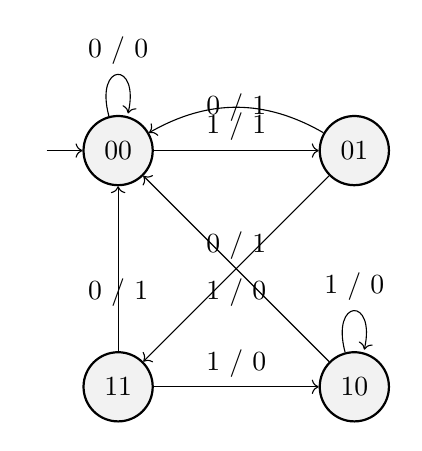
\begin{tikzpicture}
    \node[state, initial] (s0) {00};
    \node[state, right of=s0] (s1) {01};
    \node[state, below of=s1] (s2) {10};
    \node[state, below of=s0] (s3) {11};

    \draw
    (s0) edge[loop above] node{0 / 0} (s0)
    (s0) edge[above] node{1 / 1} (s1)
    (s1) edge[bend right] node{0 / 1} (s0)
    (s1) edge[below] node{1 / 0} (s3)
    (s2) edge[above] node{0 / 1} (s0)
    (s2) edge[loop above] node{1 / 0} (s2)
    (s3) edge[below] node{0 / 1} (s0)
    (s3) edge[above] node{1 / 0} (s2)
    ;
  \end{tikzpicture}
\end{figure}




\subsection{Types of Finite State Machines}

There are two types of finite state machines and therefore two types of sequential circuits:
\begin{description}
  \item[Moore Machine]  - The output depends only on the current state.
  \item[Mealy Machine] - The output depends on both the current state and the inputs.
\end{description}

\section{State Reduction and Assignment}
\dfn{State Reduction}{
  The process of reducing  the number of states of a state machine while keeping the input-output behaviour unchanged.
}

Given the finite state machine below:
\begin{figure}[H]
  \begin{center}
    % \includegraphics[width=0.3\textwidth]{stateDiag1.png}
  \end{center}
\end{figure}



\end{document}

